\documentclass{article}
\usepackage[UTF8]{ctex}
\usepackage{pythonhighlight}
\usepackage{markdown}
\usepackage{listings}
\lstset{
    basicstyle          =   \tt,          % 基本代码风格
    identifierstyle=\color{brown!80!black},
    keywordstyle        =   \color{purple}\bfseries,          % 关键字风格
    commentstyle        =   \rmfamily\itshape,  % 注释的风格,斜体
    stringstyle         =   \ttfamily,  % 字符串风格
    flexiblecolumns,                % 别问为什么,加上这个
    numbers             =   left,   % 行号的位置在左边
    showspaces          =   false,  % 是否显示空格,显示了有点乱,所以不现实了
    numberstyle         =   \zihao{-5}\ttfamily,    % 行号的样式,小五号,tt等宽字体
    showstringspaces    =   false,
    captionpos          =   t,      % 这段代码的名字所呈现的位置,t指的是top上面
    frame               =   lrtb,   % 显示边框
    backgroundcolor=\color[RGB]{245,245,244},
}


% Language setting
% Replace `english' with e.g. `spanish' to change the document language
\usepackage[english]{babel}
\usepackage{float}
% Set page size and margins
% Replace `letterpaper' with `a4paper' for UK/EU standard size
\usepackage[letterpaper,top=2cm,bottom=2cm,left=3cm,right=3cm,marginparwidth=1.75cm]{geometry}

% Useful packages
\usepackage{amsmath}
\usepackage{graphicx}
\usepackage[colorlinks=true, allcolors=blue]{hyperref}

\title{数逻实验报告Lab8}
\author{雷远航}

\begin{document}
    
\maketitle

\begin{abstract}
    加法器、加减法器和ALU 
\end{abstract}

\section*{一:操作方法与实验步骤}

\subsection*{任务一:原理图设计4位加减法器}

\subsubsection*{实现一位全加器:}
根据一位全加器的布尔函数值绘制其原理图
\begin{figure}[H]
    \centering
    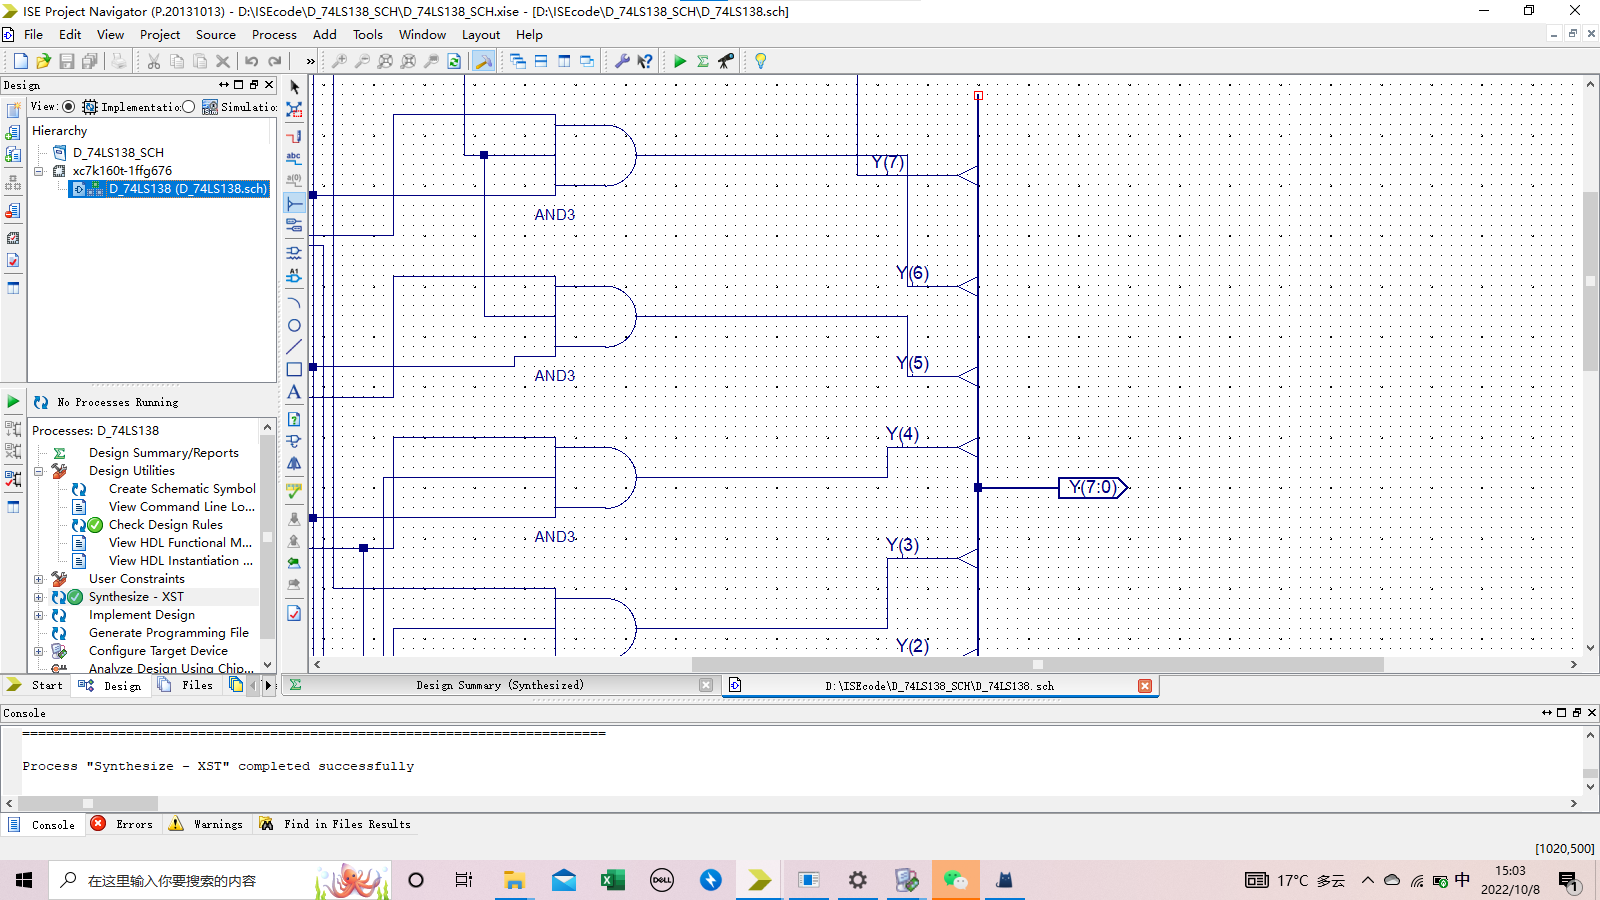
\includegraphics[width=0.9\textwidth]{lab8/1.png}
    \caption{\label{Lab8}一位全加器}
    \end{figure}

\subsubsection*{实现4位加减法器:}
首先实现一个一位加减法器,在此基础上实现四位加减法器.
\begin{figure}[H]
    \centering
    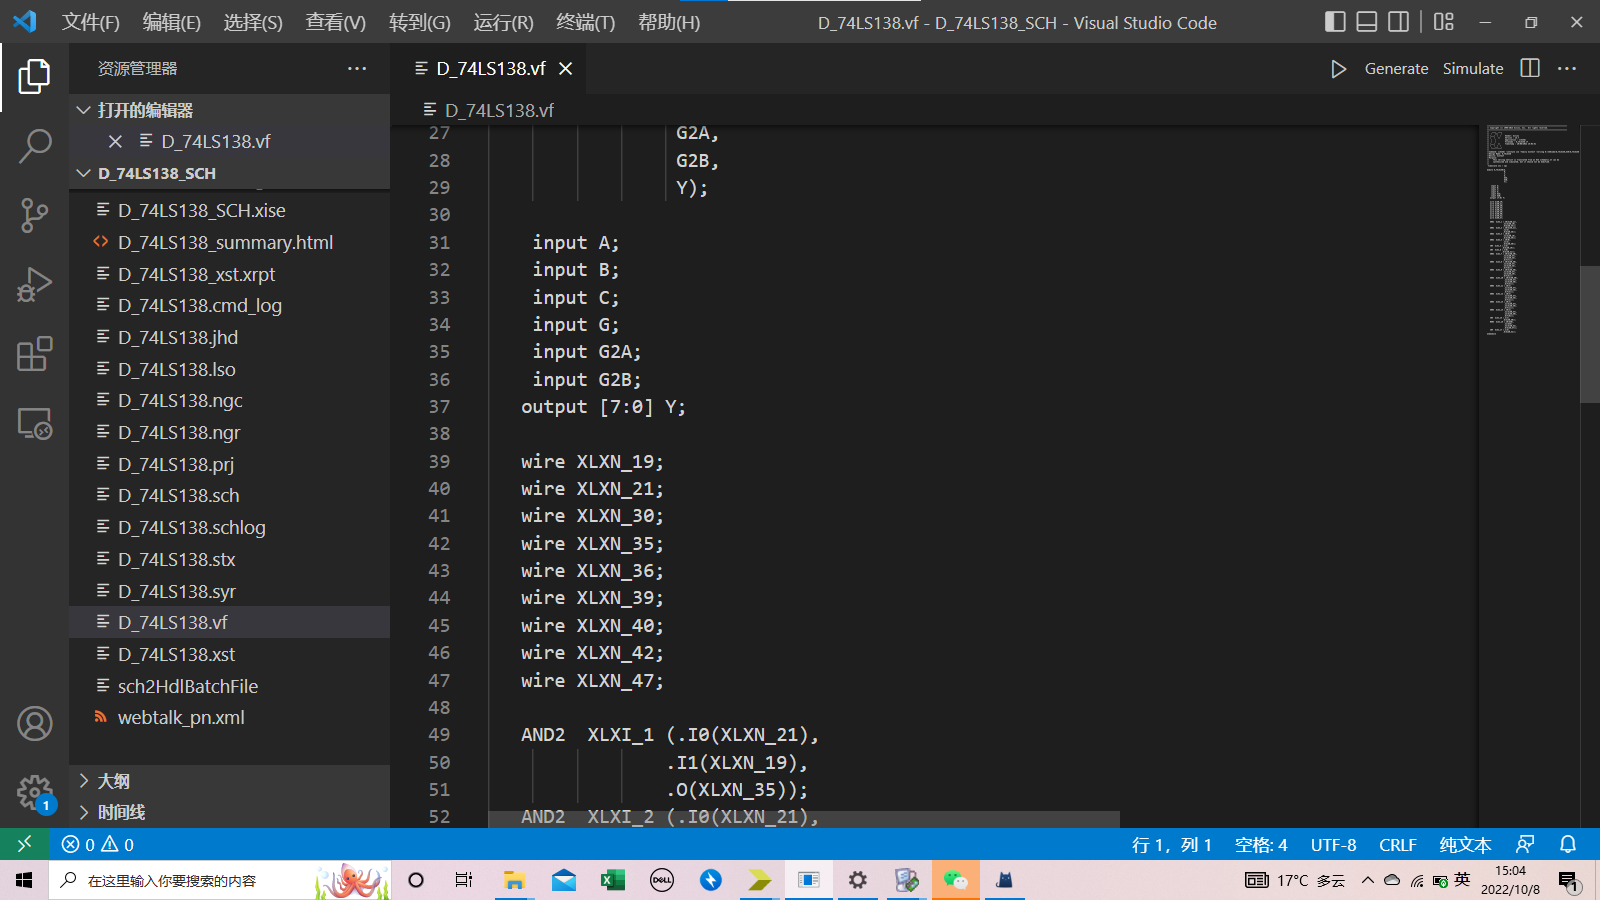
\includegraphics[width=0.9\textwidth]{lab8/2.png}
    \caption{\label{Lab8}一位加减法器}
    \end{figure}

在一位加减法器的基础上通过串行实现四位加减法器. 
    \begin{figure}[H]
    \centering
    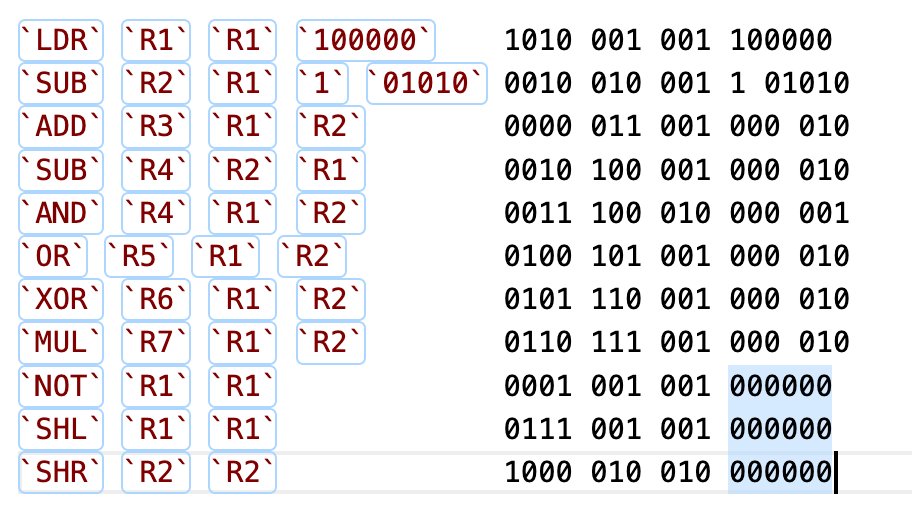
\includegraphics[width=0.6\textwidth]{lab8/3.png}
    \caption{\label{Lab8}四位加减法器}
    \end{figure}

对实现的四位加减法器进行模拟仿真,对边界条件进行测试,仿真激励代码如下:
\begin{lstlisting}[language=verilog]
    `timescale 1ns / 1ps

    module AddSub4b_AddSub4b_sch_tb();
    
    // Inputs
       reg [3:0] A;
       reg [3:0] B;
       reg Ctrl;
    
    // Output
       wire [3:0] S;
       wire Co;
    
    // Bidirs
    
    // Instantiate the UUT
       AddSub4b UUT (
            .A(A), 
            .B(B), 
            .Ctrl(Ctrl), 
            .S(S), 
            .Co(Co)
       );
    // Initialize Inputs
       
           initial begin
          A = 4'b0001;
            B = 4'b0011;
            Ctrl = 1;//overflow
          #30;
            A = 4'b1111;
            B = 4'b1111;
            Ctrl = 0;//overflow
          #30;
          A = 4'b1111;
          B = 4'b1111;
          Ctrl = 1;
          #30;
          A = 4'b1001;
          B = 4'b0110;
          Ctrl = 0;
          #30;
          A = 4'b1001;
          B = 4'b0110;
          Ctrl = 1;
          #30;
          A = 4'b1111;
          B = 4'b0001;
          Ctrl = 0;   //overflow 
          #30;
          A = 4'b0001;
          B = 4'b0010;
          Ctrl = 1;
    
           end
    endmodule
    
\end{lstlisting}

\subsection*{任务2:实现4位ALU及应用设计}

用原理图方式绘制ALU,利用已经绘制好的四位与门、四位或门和MUX模块.
    \begin{figure}[H]
    \centering
    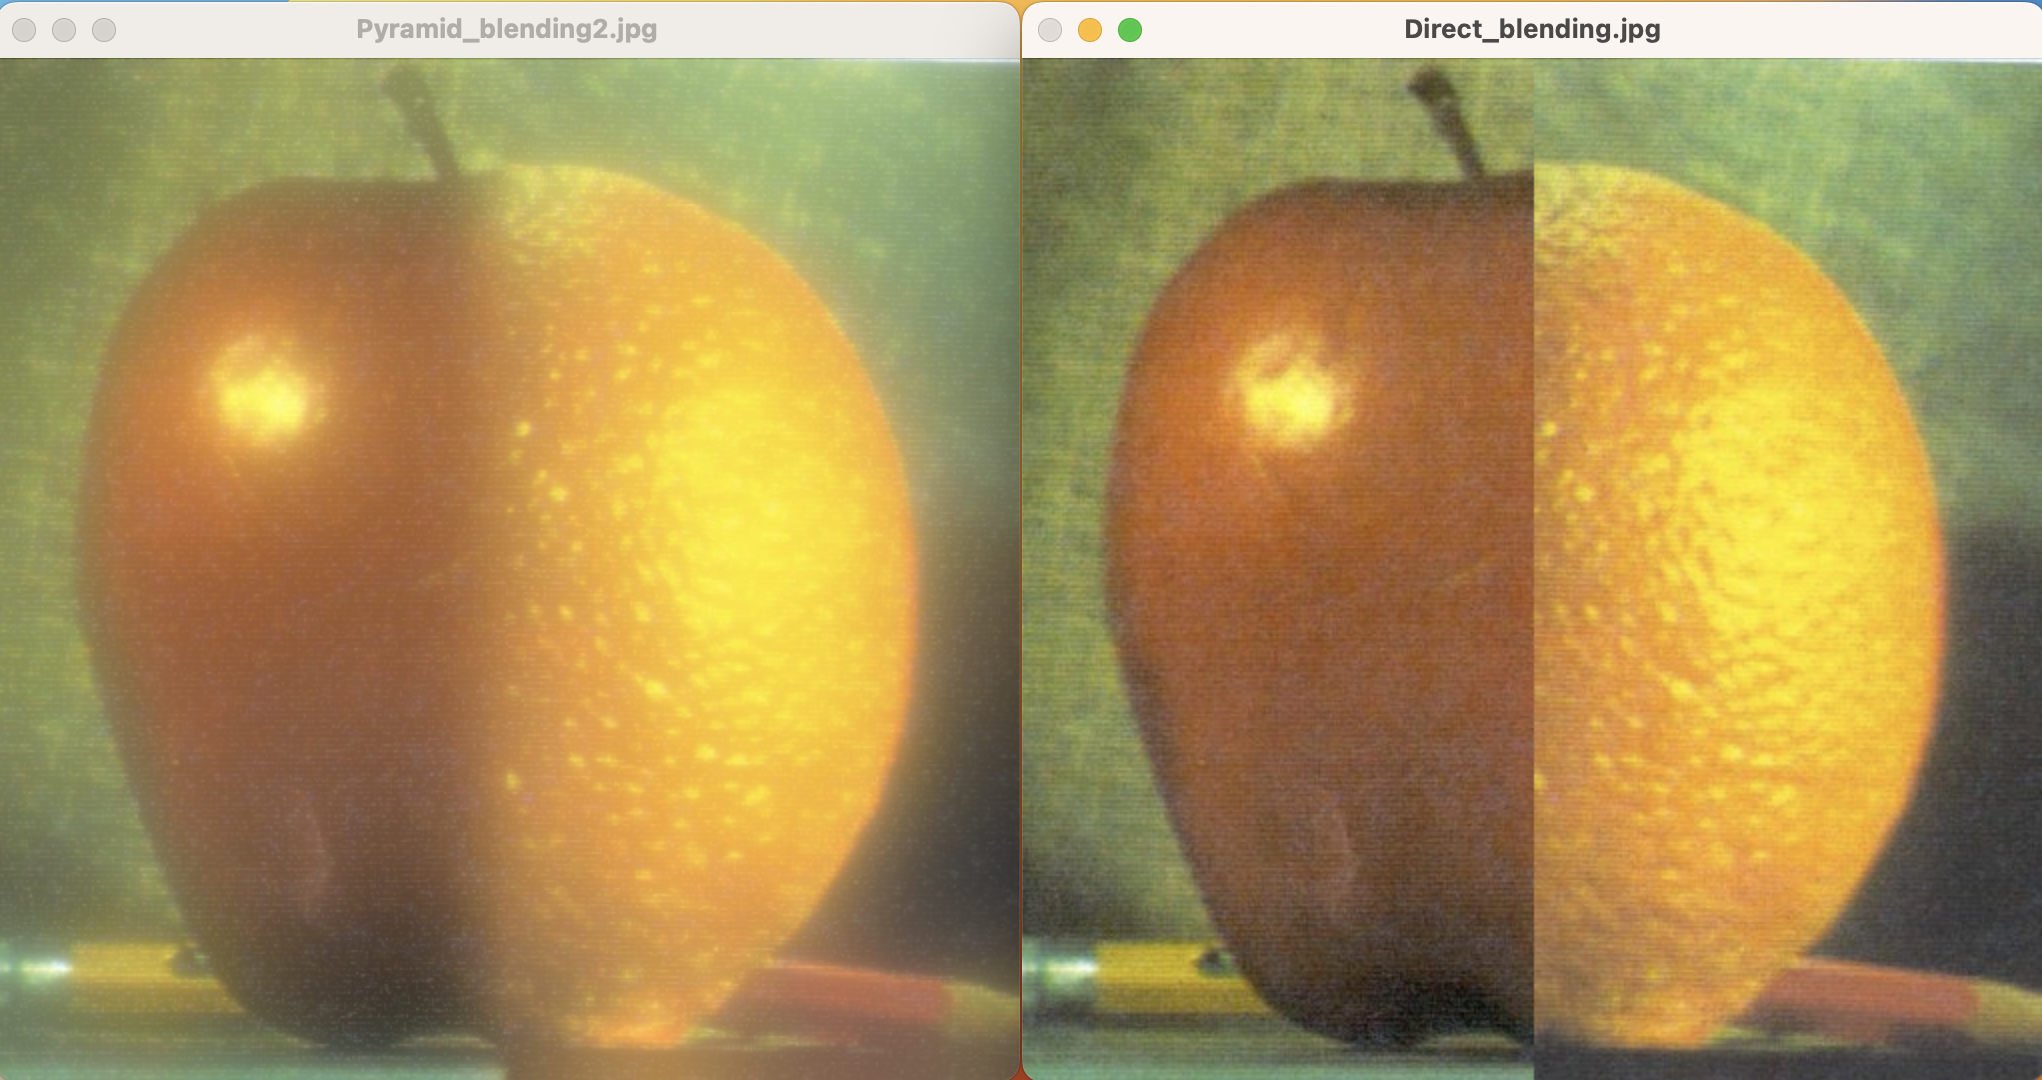
\includegraphics[width=0.9\textwidth]{lab8/5.png}
    \caption{\label{Lab8}ALU}
    \end{figure}

导入top.v和IP核中的内容,以及附件中的防抖动模块和clk模块等,并且将top.v中相关的信息填充完整,
同时完成Sseg\_Dev模块的绘制.
\begin{figure}[H]
    \centering
    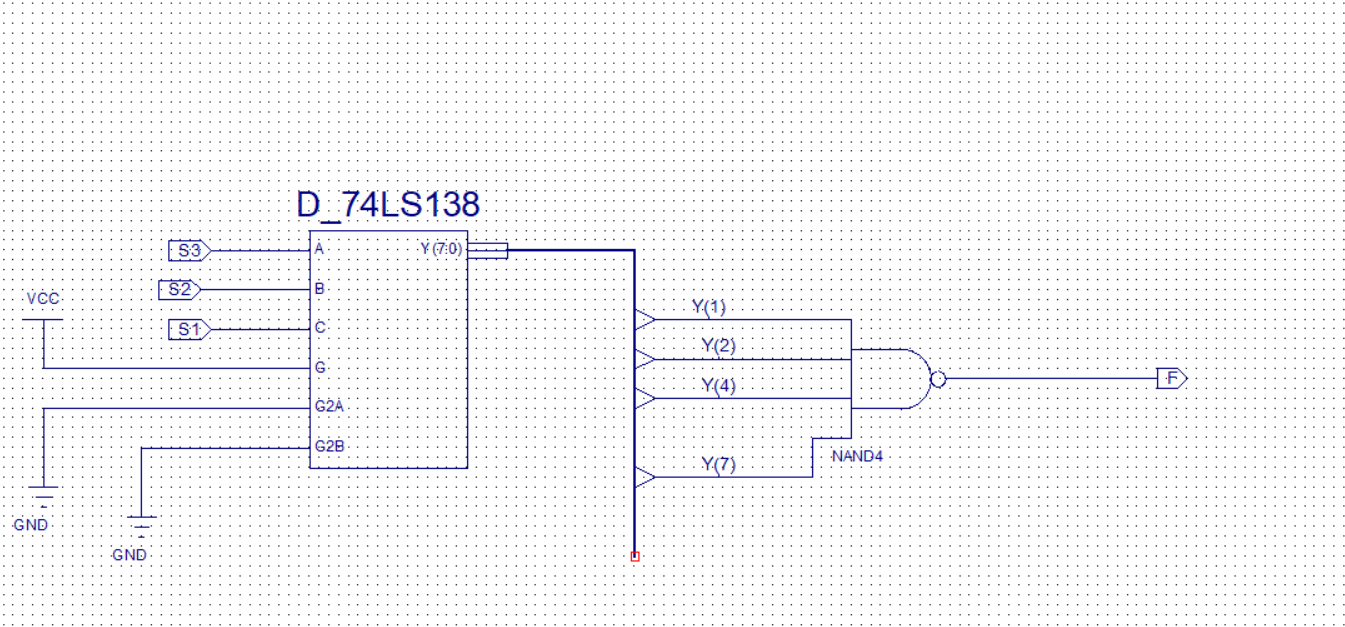
\includegraphics[width=0.9\textwidth]{lab8/7.png}
    \caption{\label{Lab8}Sseg\_Dev}
    \end{figure}
    
对ALU模块进行模拟仿真,并且对边界条件进行测试,仿真激励代码如下:
\begin{lstlisting}[language=verilog]
    `timescale 1ns / 1ps

    module ALU_ALU_sch_tb();
    
    // Inputs
       reg [3:0] A;
       reg [3:0] B;
       reg [1:0] S;
    
    // Output
       wire [3:0] C;
       wire Co;
    
    // Bidirs
    
    // Instantiate the UUT
       ALU UUT (
            .A(A), 
            .B(B), 
            .S(S), 
            .C(C), 
            .Co(Co)
       );
    // Initialize Inputs
       integer i;
           initial begin
            A = 4'b1111;
            B = 4'b0000;
            for (i=0; i<=3; i=i+1) begin
             {S[1:1],S[0:0]} <= i;
             #30;
          end
          #20
          A = 4'b1001;
            B = 4'b0110;
            for (i=0; i<=3; i=i+1) begin
             {S[1:1],S[0:0]} <= i;
             #30;
          end
          A = 4'b1111;
            B = 4'b0001;
            for (i=0; i<=3; i=i+1) begin
             {S[1:1],S[0:0]} <= i;
             #30;
          end
          A = 4'b0111;
            B = 4'b1000;
            for (i=0; i<=3; i=i+1) begin
             {S[1:1],S[0:0]} <= i;
             #30;
          end
          A = 4'b0001;
            B = 4'b0010;
            for (i=0; i<=3; i=i+1) begin
             {S[1:1],S[0:0]} <= i;
             #30;
          end
           end
    endmodule
\end{lstlisting}


\section*{二:实验结果与分析}

\subsection*{AddSub4b模拟仿真结果分析:}
\subsubsection*{波形图如下:}    
    \begin{figure}[H]
    \centering
    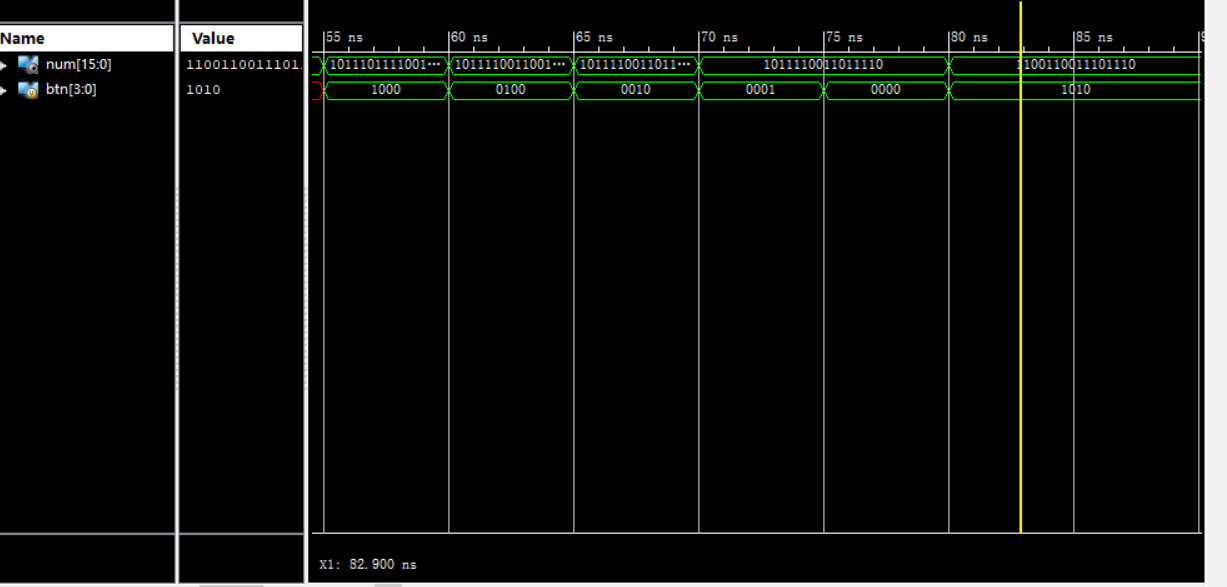
\includegraphics[width=0.9\textwidth]{lab8/8.png}
    \caption{\label{Lab8}AddSub4b波形图}
    \end{figure}
\subsubsection*{结果分析:}
Ctrl为1时代表进行减法,Ctrl为0时代表进行加法.

第一组数据是一个边界条件数据:1-3,发生了overflow,因此Co位的结果为1,代表overflow的发生,最终的结果表示减数取反加1与被减数相加的结果,可以验证结果是正确的.

第二组数据也是一个边界条件数据:15+15,加法发生的overflow,最终的实际结果不能由四位的二进制数进行表示,Co为有一个进位,代表发生了overflow,最终S[3:0]的结果也是正确的.

第三组数据是:15-15,最终的结果是0,没有overflow的发生,因此Co为0.

第四组、第五组的数据是:9+6与9-6,最终的结果是15和3,同样也是正确的.

第六组是一个边界数据:15+1,发生了加法的overflow,因此Co为1,S为0.

第七组是边界数据:1-2,发生减法的overflow,Co为1,S为15.


\subsection*{ALU波形图分析和下版结果:}
   
\subsubsection*{波形图:}
    \begin{figure}[H]
    \centering
    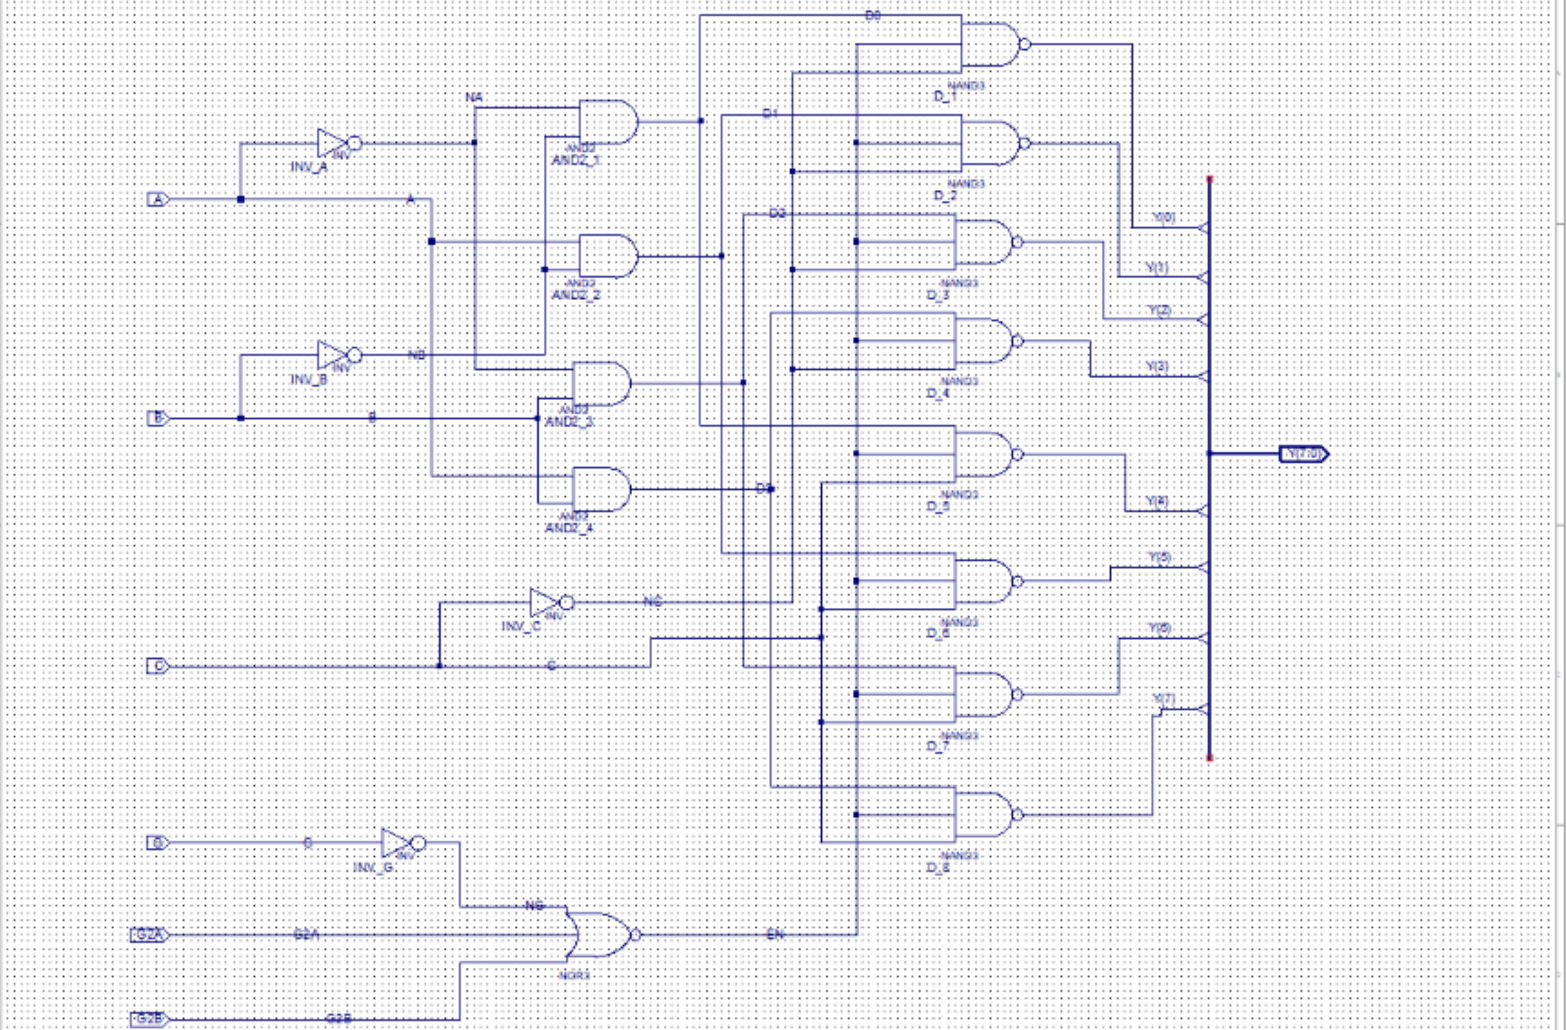
\includegraphics[width=0.9\textwidth]{lab8/9.png}
    \caption{\label{Lab8}ALU波形图}
    \end{figure}
\subsubsection*{波形图分析:}
对于每一组数据,对S[1:0]从0到3遍历,对数据一次执行加、减、与、或的四个操作.

第一组数据:4'b1111与4'0000进行运算,加法的结果是15,减法的结果是15,与运算为4'b0000,或运算为4'b1111.

第二组数据:4'b1001与4'b0110进行运算,加、减、与、或的结果分别是:15,3,4'b0000,4'b1111.这是一组对与、或运算边界情况的运算.

第三组数据:4'b1111和4'b0001,加、减、与、或的结果分别是:0,14,1,15.这是一个对加法运算的边界数据:加法发生了overflow,因此Co位为1.

第四组数据:4'b0111和4'b1000,加、减、与、或的结果分别是:15,15,0,15.这是一个对减法运算的边界数据,在减法执行时用较小的数减去较大的数,发生了overflow,因此Co为1.

第五组数据:1和2,加、减、与、或的结果分别是:3,15,0,3.这是一个对减法运算的边界数据,在减法执行时用较小的数减去较大的数,发生了overflow,因此Co为1.

\subsubsection*{下版结果:}
    \begin{figure}[H]
    \centering
    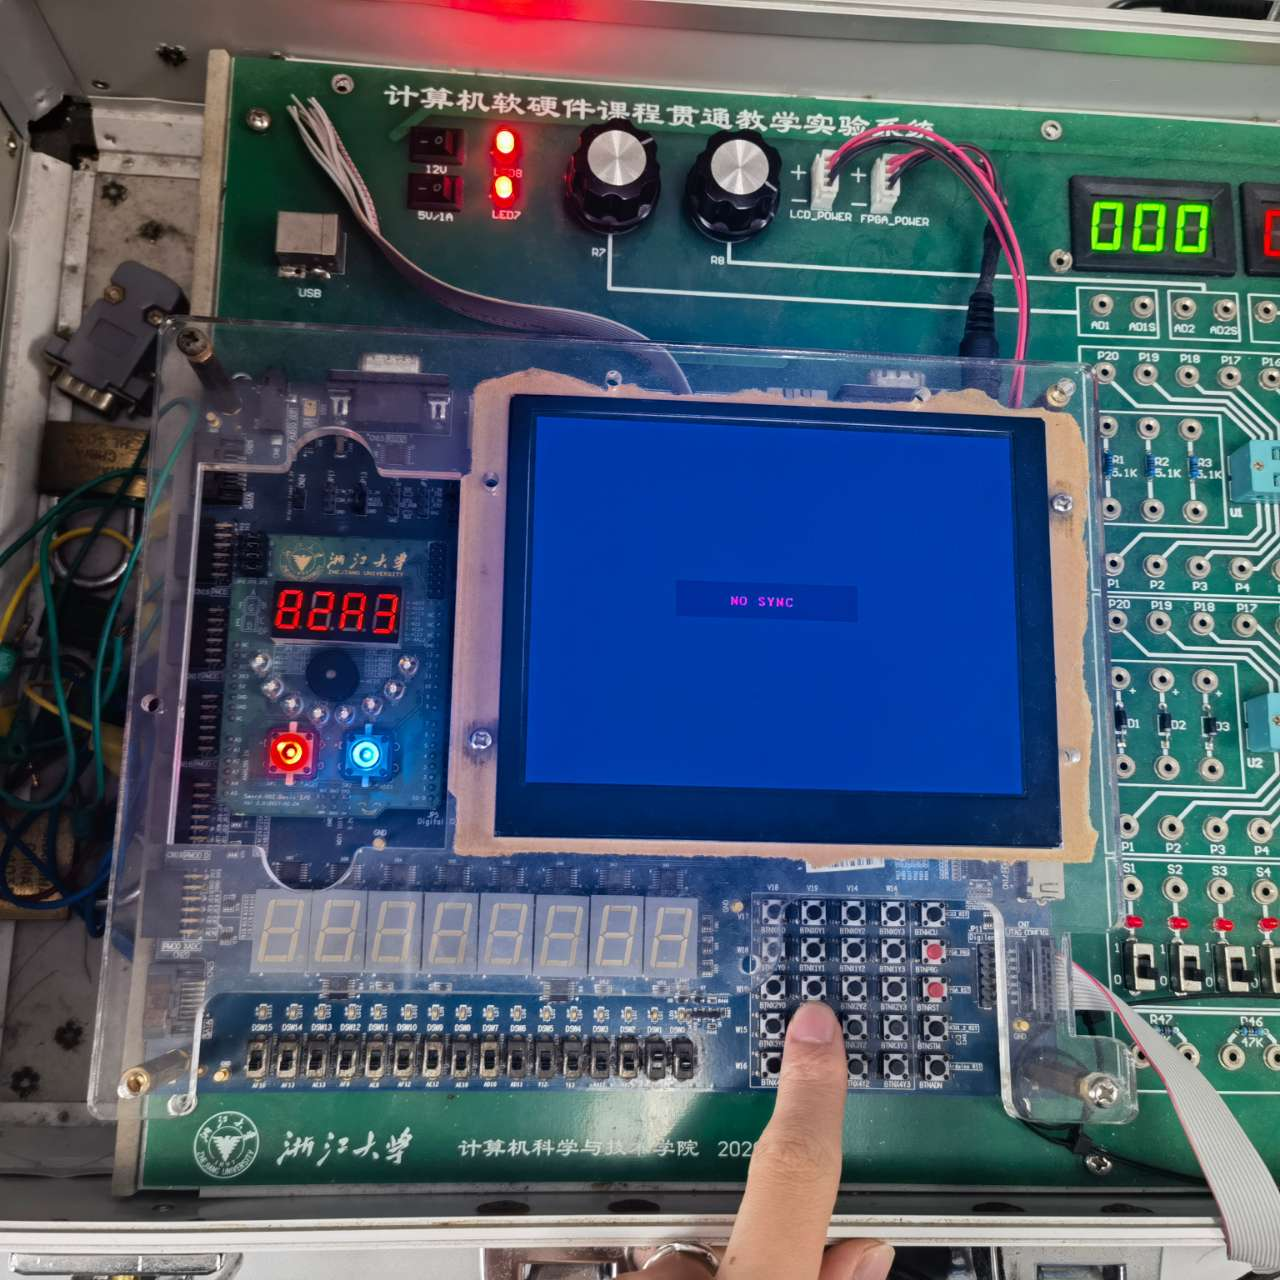
\includegraphics[width=0.5\textwidth]{lab8/11.jpg}
    \caption{\label{Lab8}4+2}
    \end{figure}

    \begin{figure}[H]
    \centering
    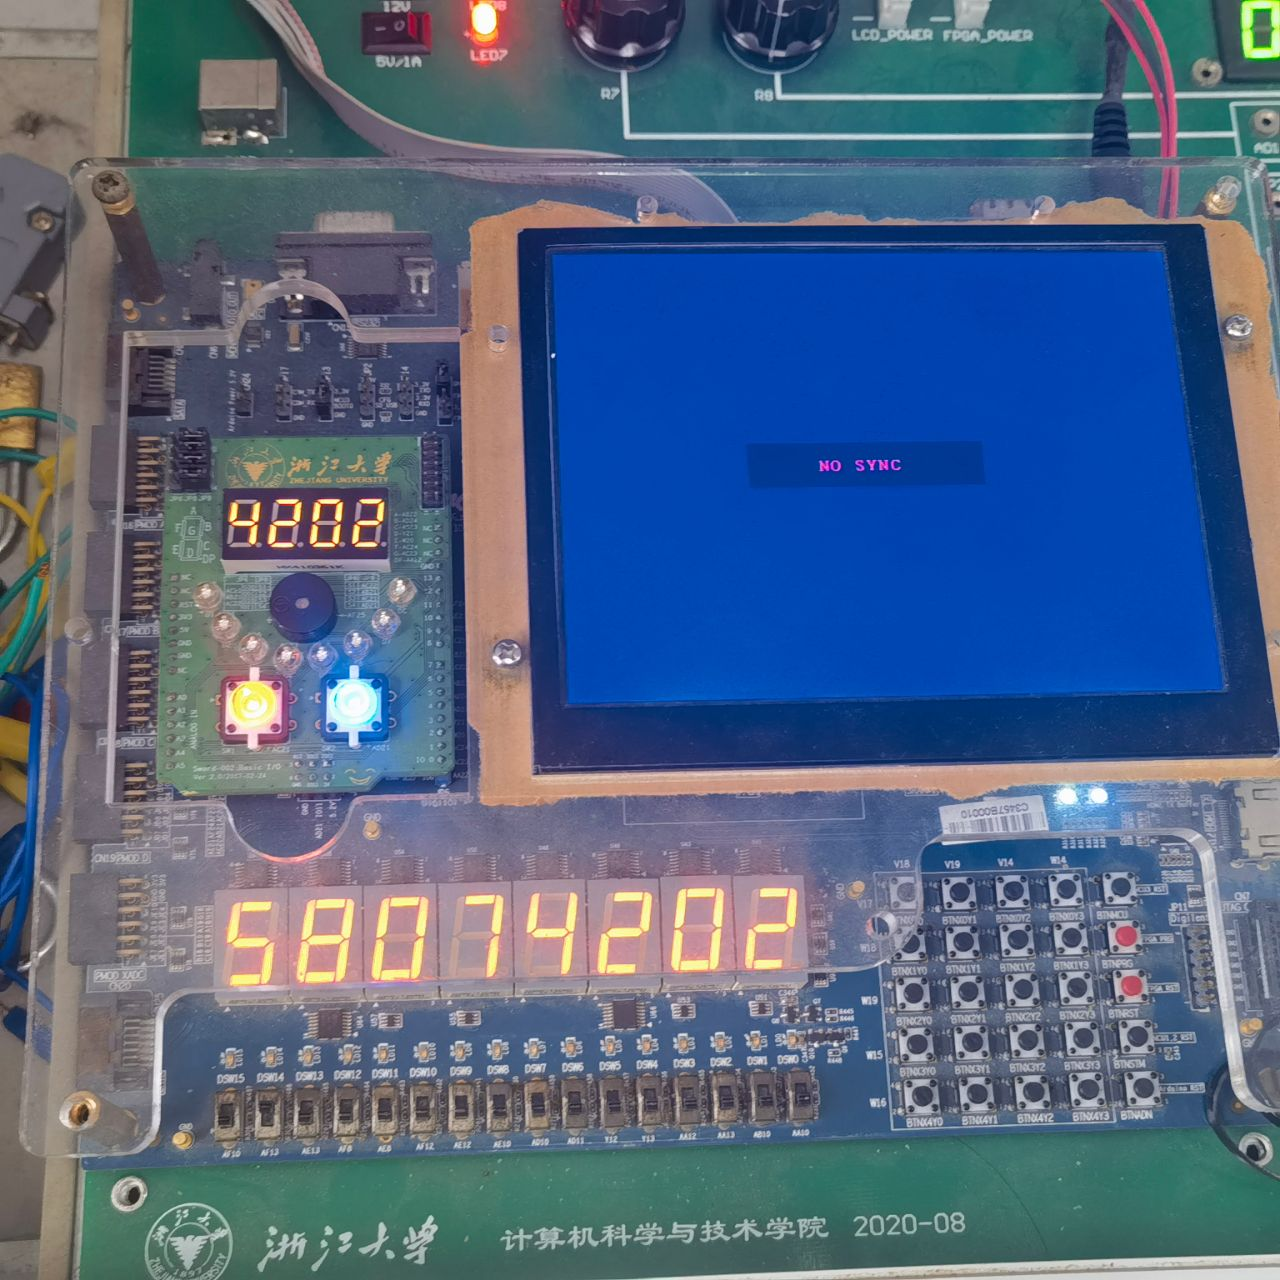
\includegraphics[width=0.5\textwidth]{lab8/12.jpg}
    \caption{\label{Lab8}4-2}
    \end{figure}

    \begin{figure}[H]
    \centering
    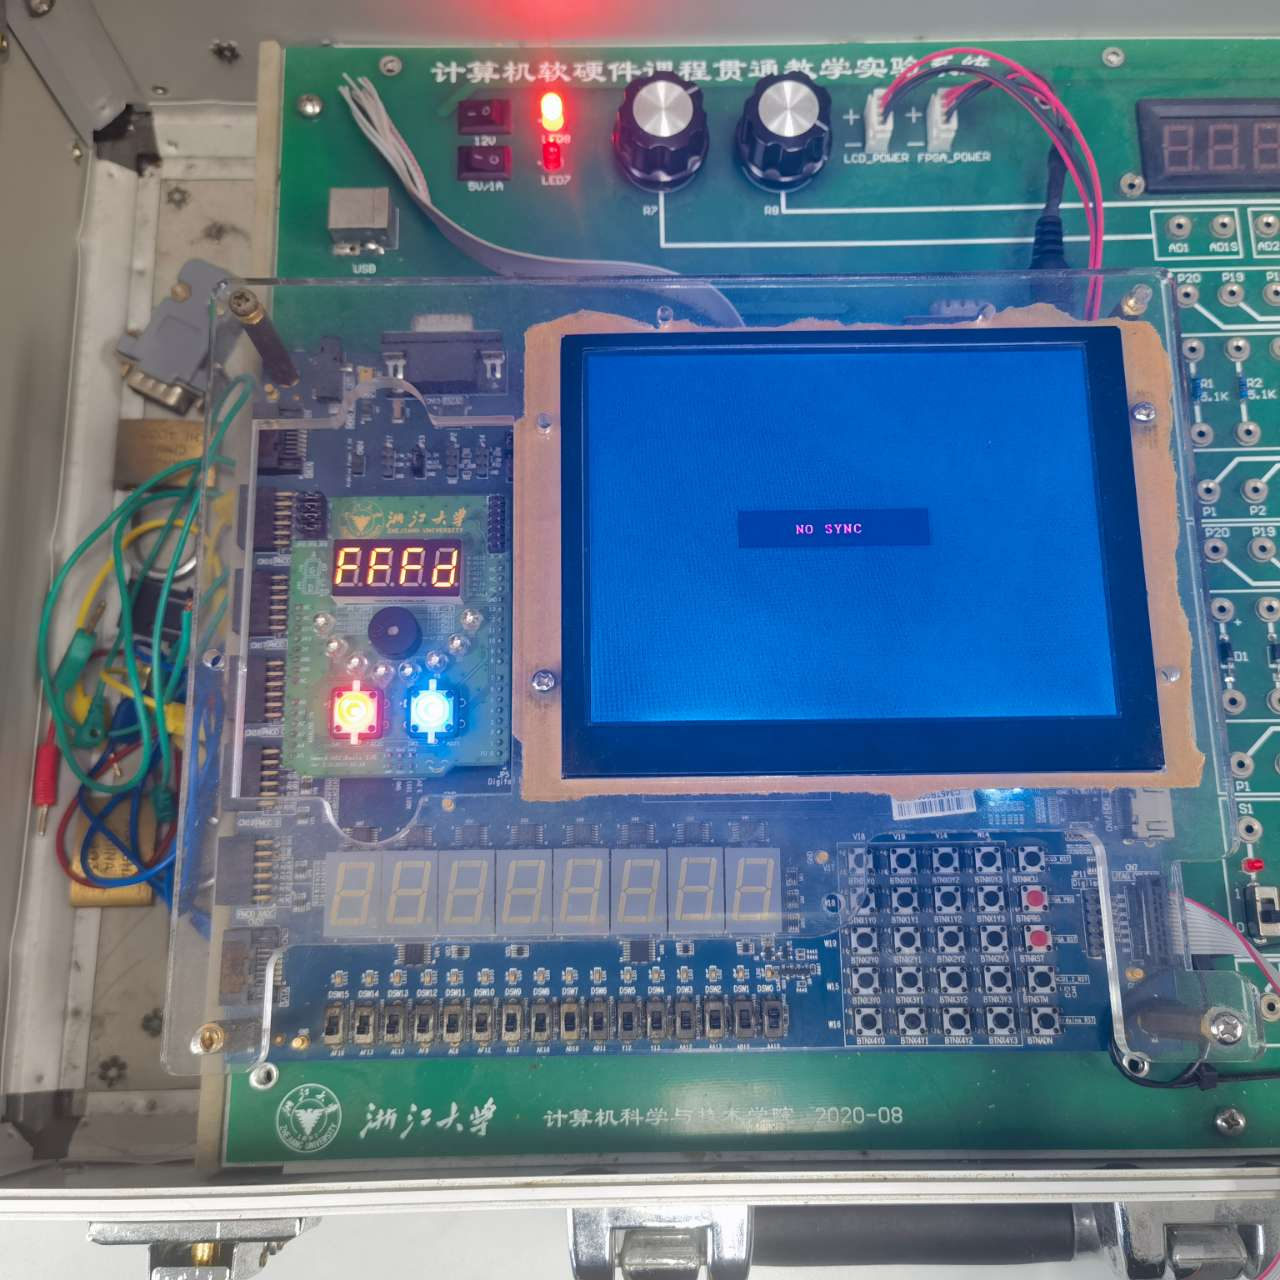
\includegraphics[width=0.5\textwidth]{lab8/13.jpg}
    \caption{\label{Lab8}4\&2}
    \end{figure}

    \begin{figure}[H]
    \centering
    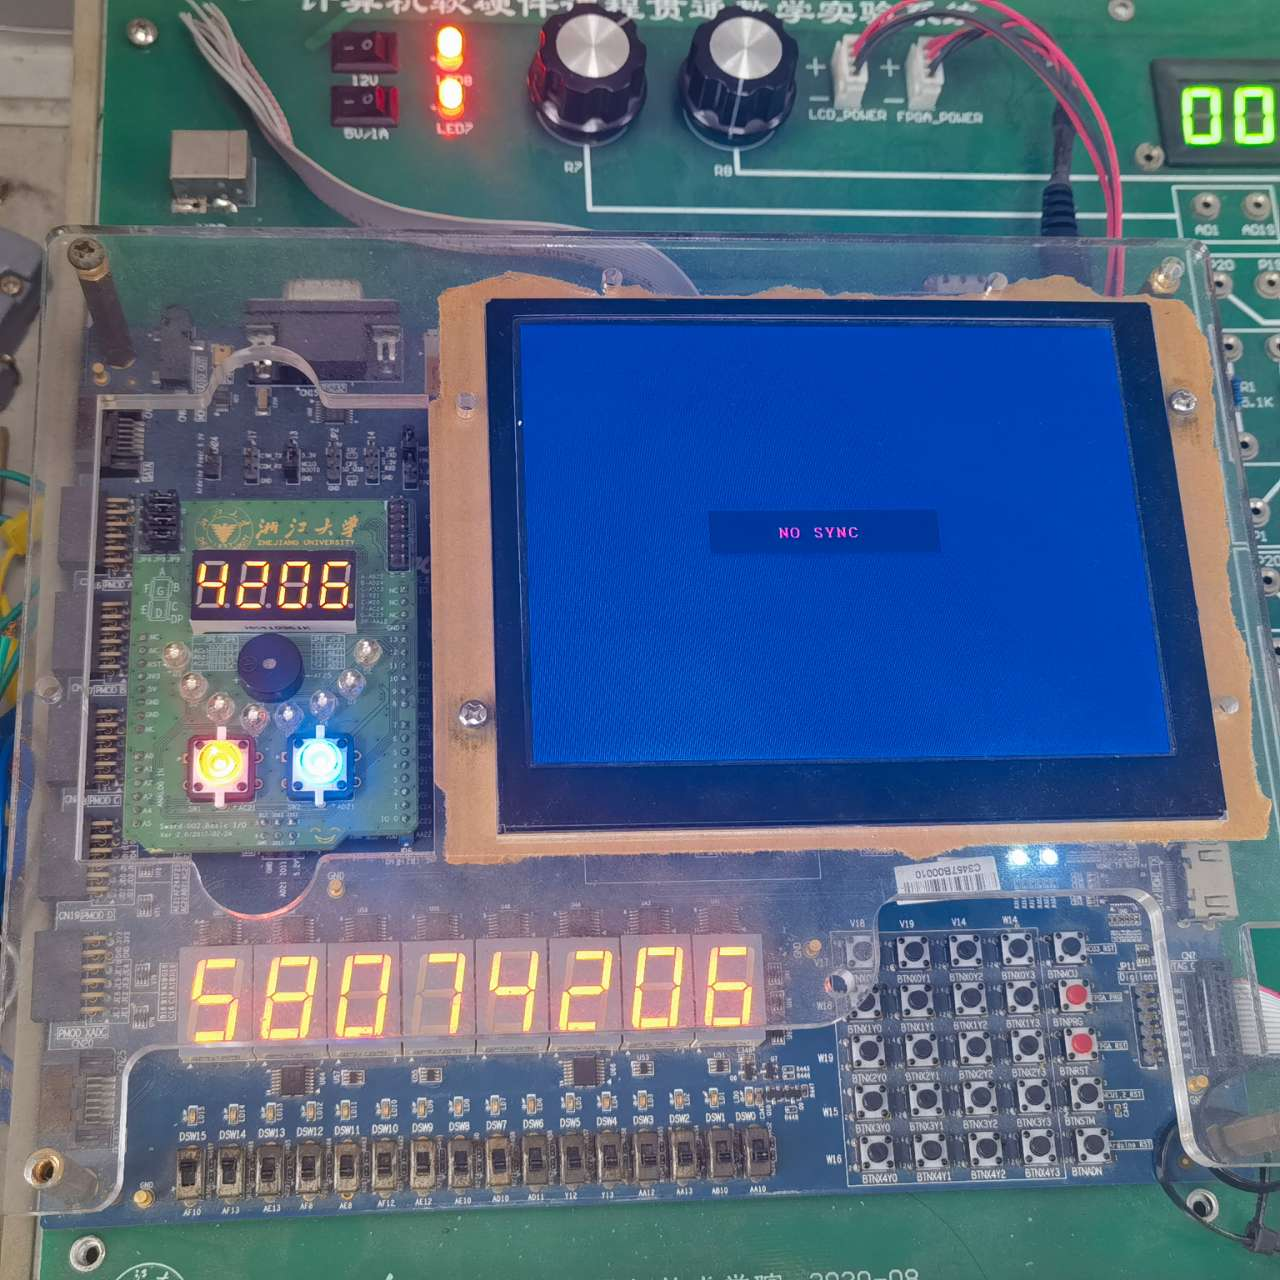
\includegraphics[width=0.5\textwidth]{lab8/14.jpg}
    \caption{\label{Lab8}4|2}
    \end{figure}

    \begin{figure}[H]
    \centering
    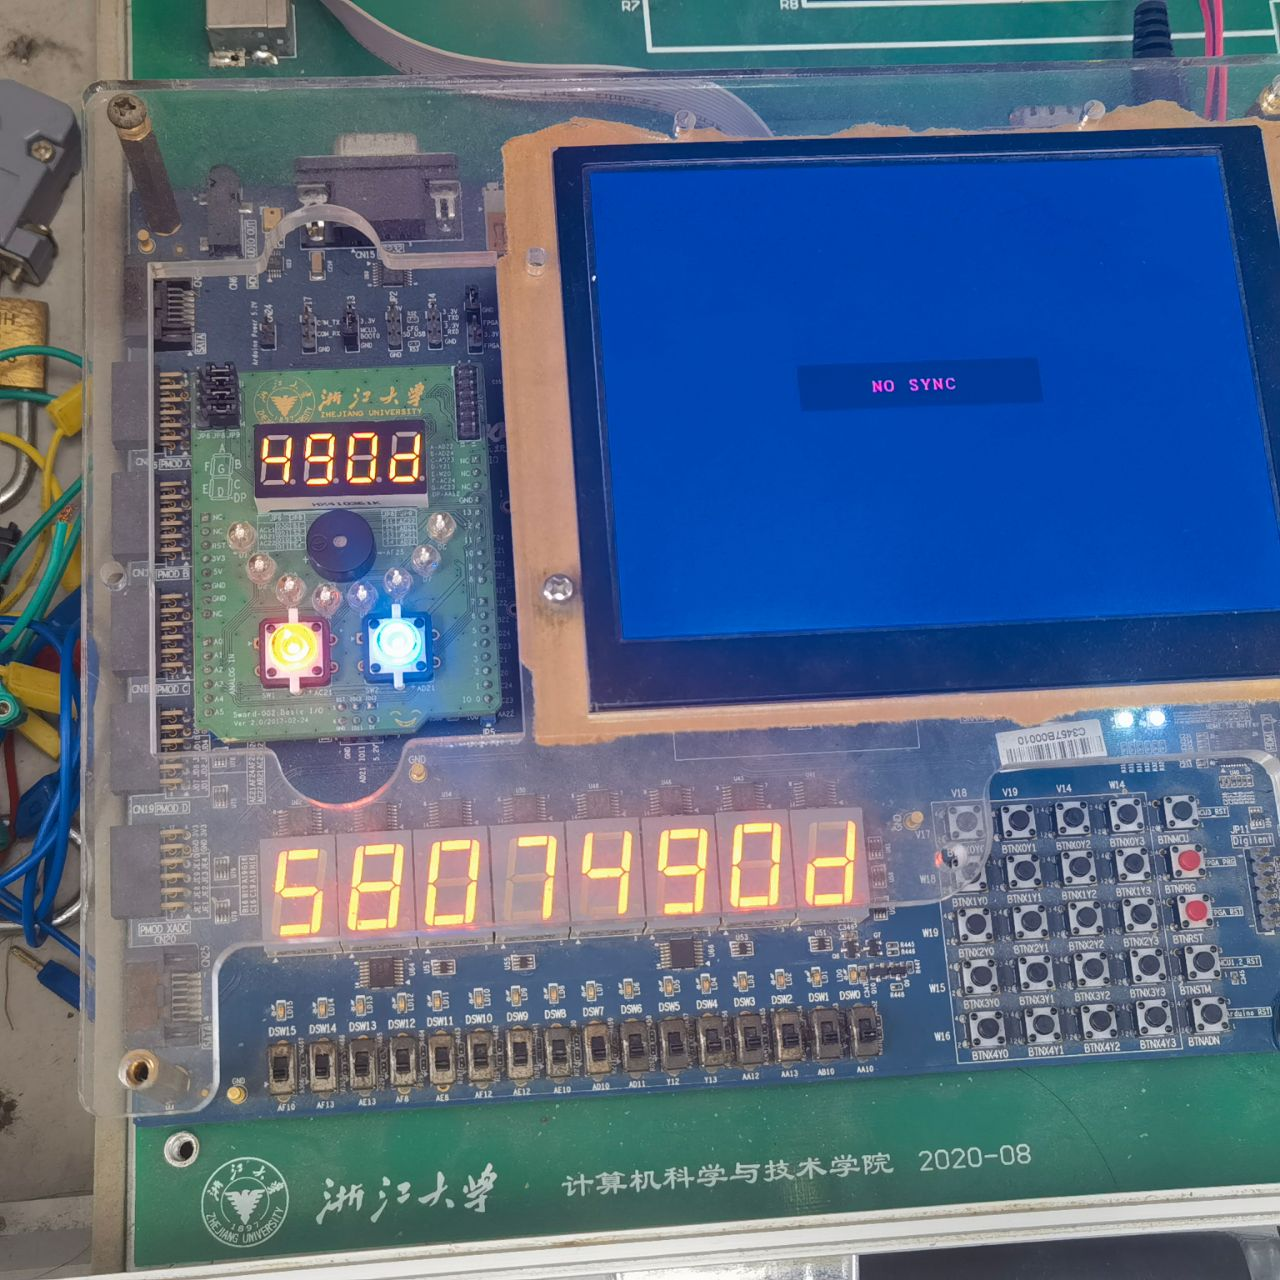
\includegraphics[width=0.5\textwidth]{lab8/16.jpg}
    \caption{\label{Lab8}4+9}
    \end{figure}

    \begin{figure}[H]
    \centering
    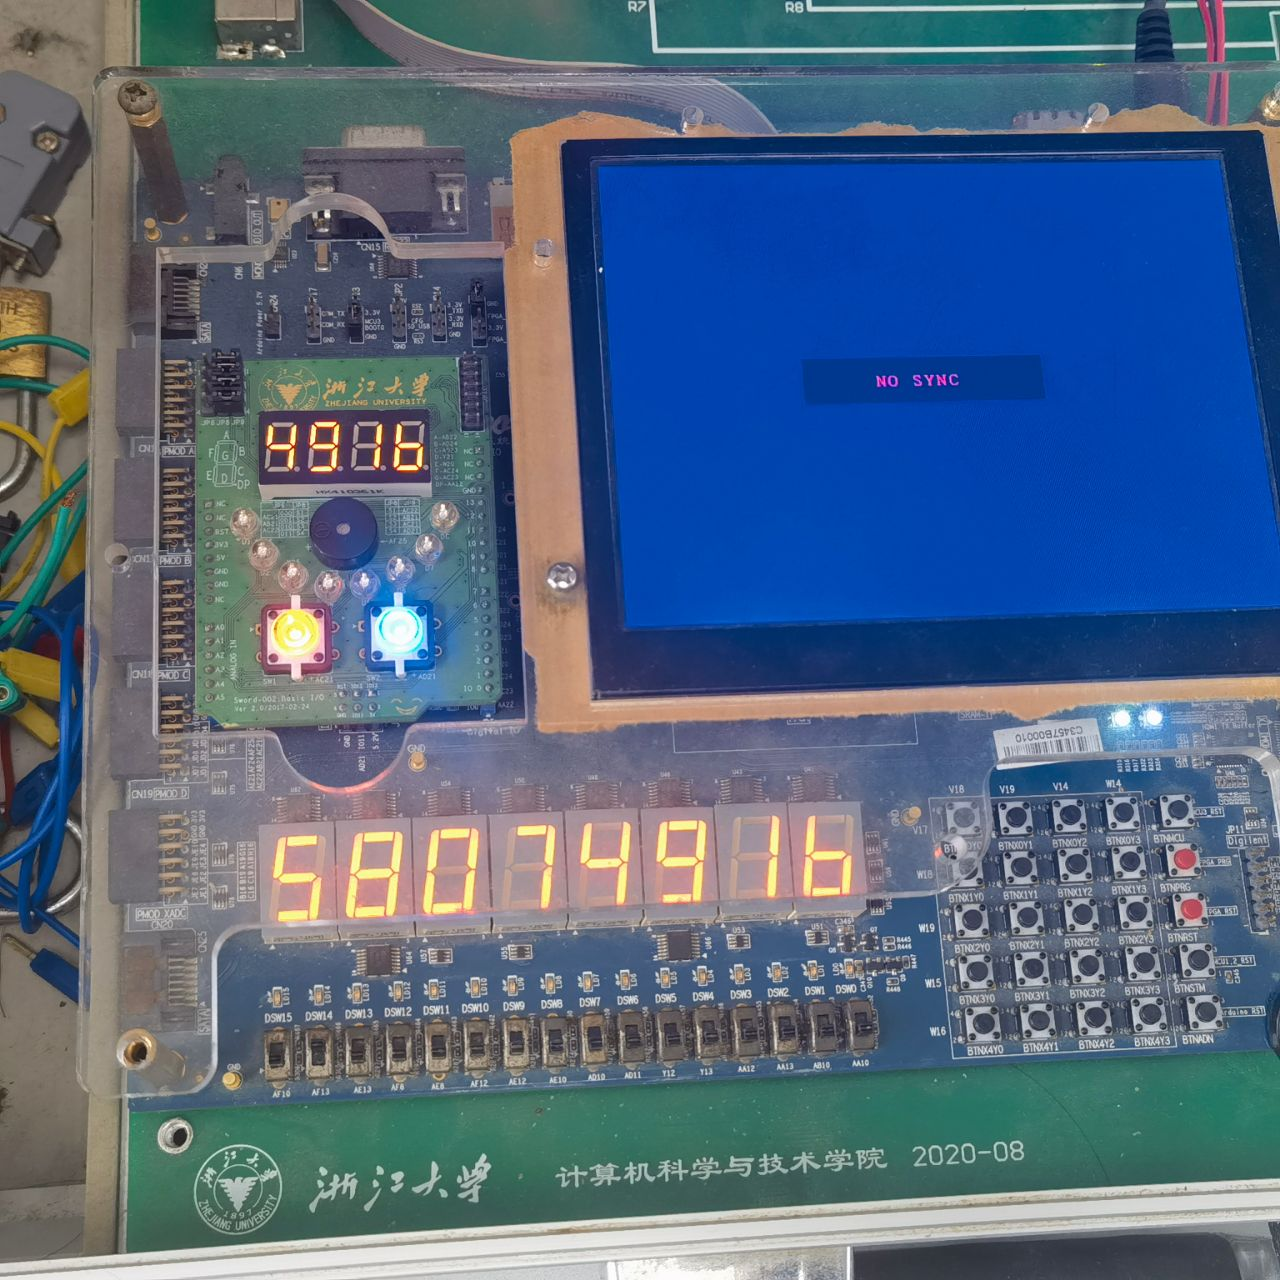
\includegraphics[width=0.5\textwidth]{lab8/17.jpg}
    \caption{\label{Lab8}4-9}
    \end{figure}

    \begin{figure}[H]
    \centering
    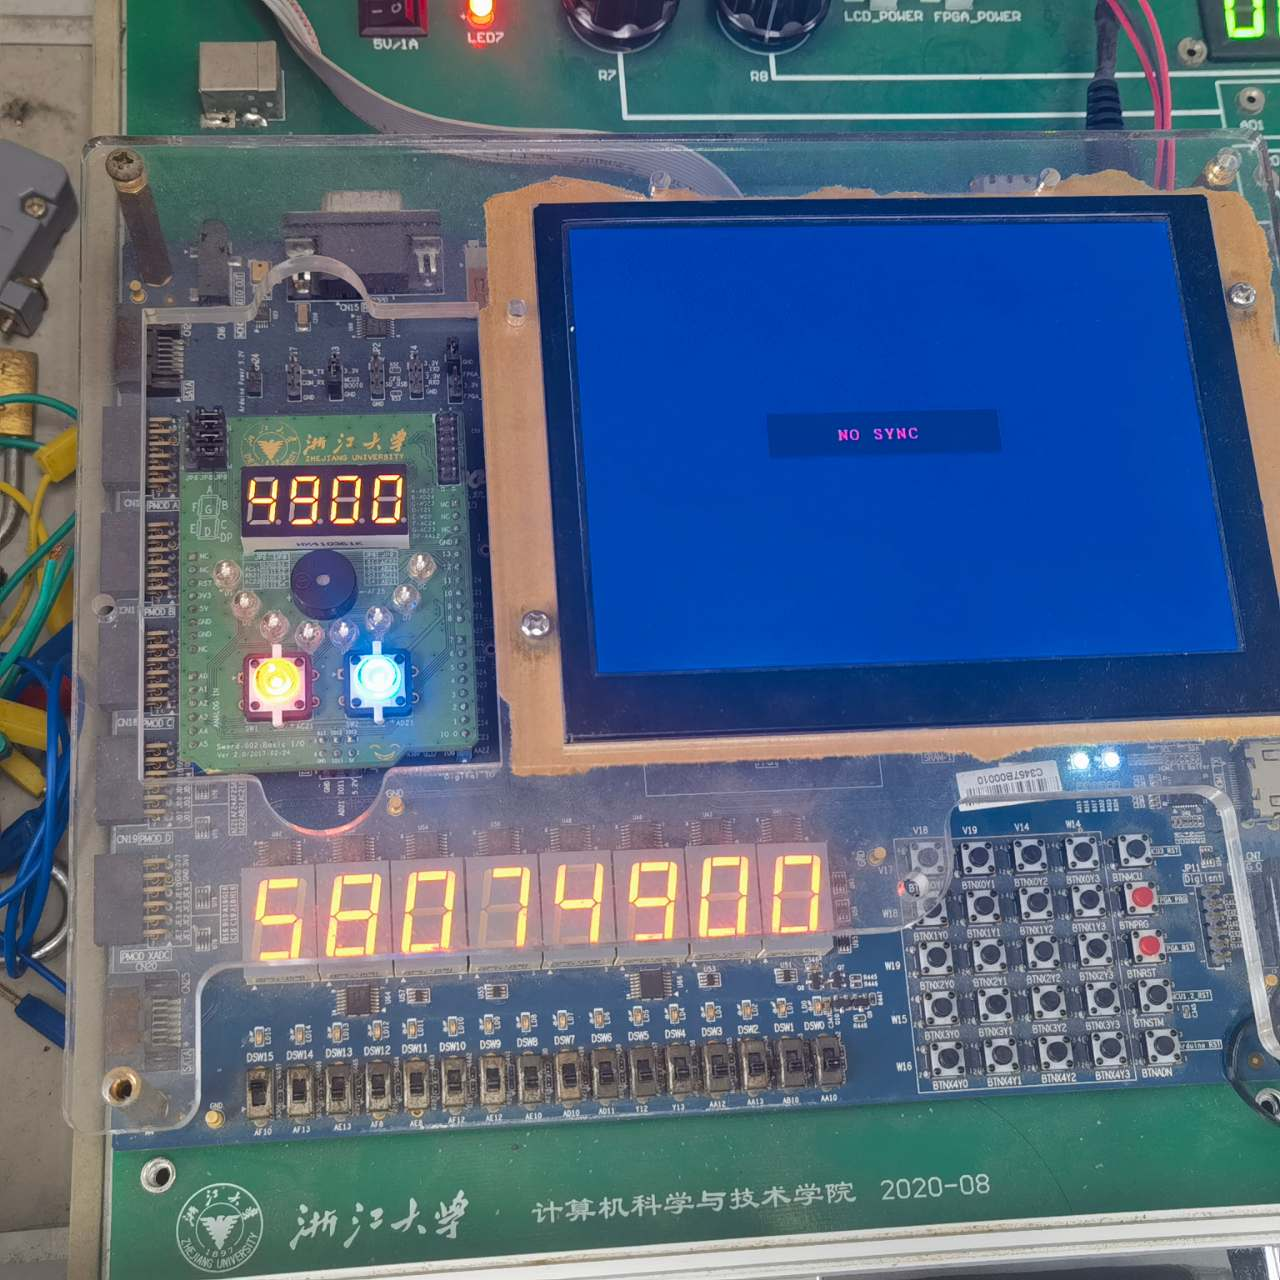
\includegraphics[width=0.5\textwidth]{lab8/18.jpg}
    \caption{\label{Lab8}4\&9}
    \end{figure}

    \begin{figure}[H]
    \centering
    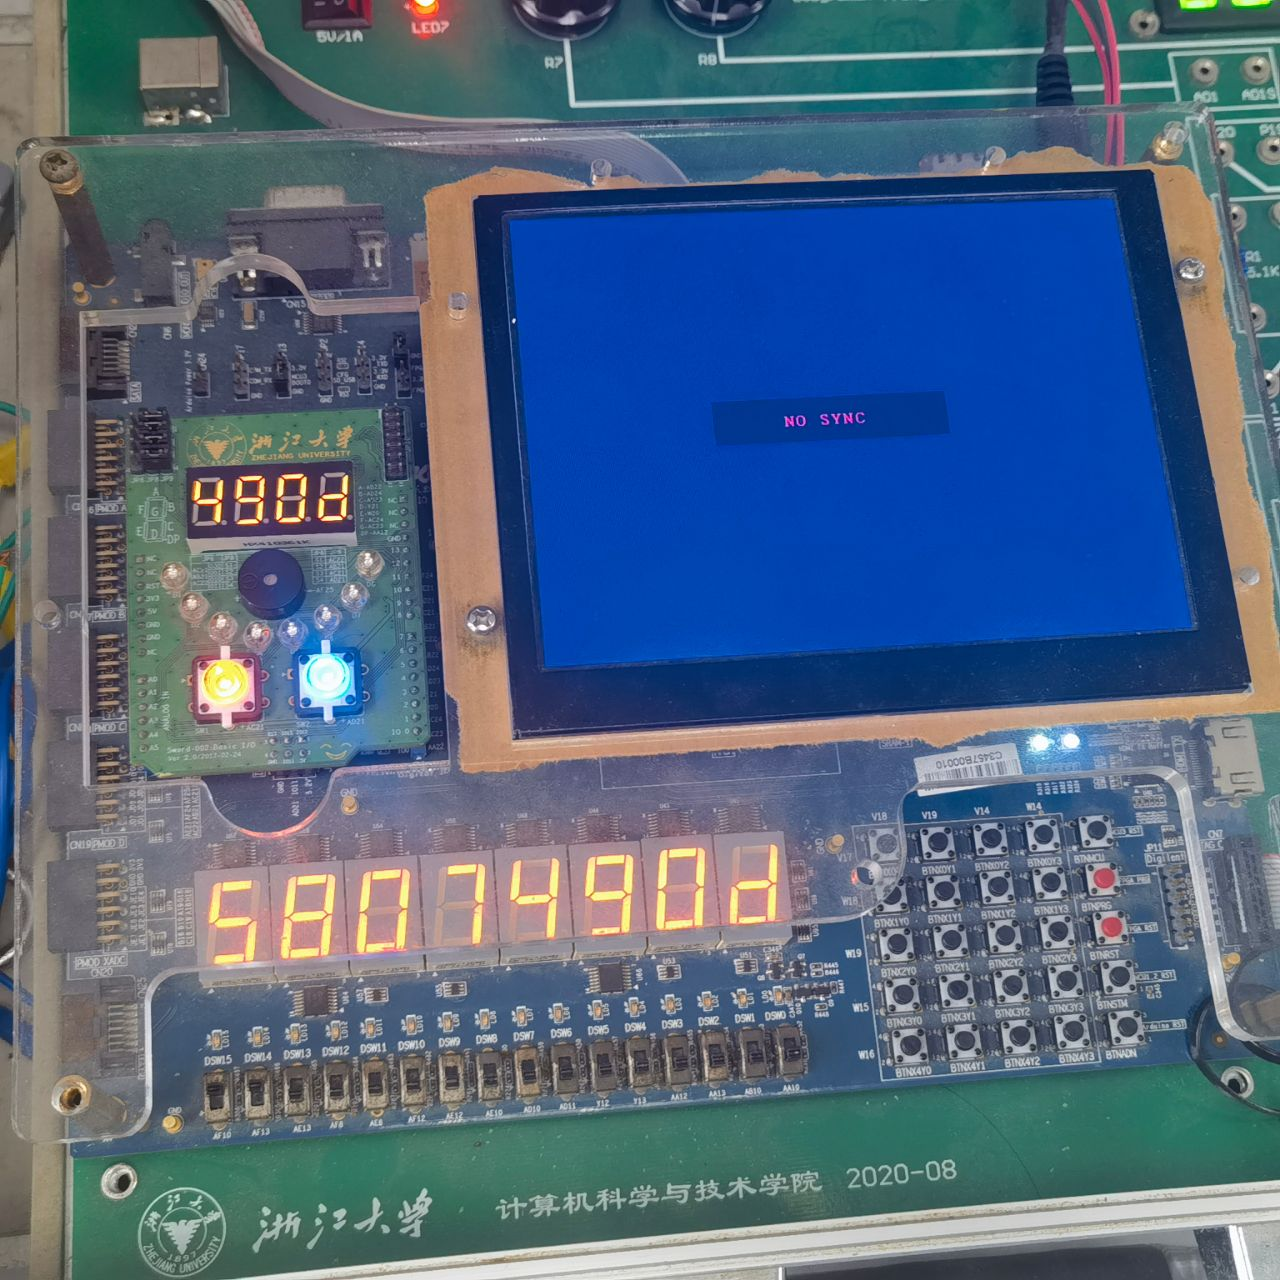
\includegraphics[width=0.5\textwidth]{lab8/19.jpg}
    \caption{\label{Lab8}4|9}
    \end{figure}

\subsubsection*{下版结果分析:}
版的前四个数是我的学号后四位.

前四组的下版数据是4与2的加、减、与、或的运算,没有发生overflow,因此倒数第二个七段数码管(代表Co)所得到的结果都是0,
加、减、与、或的结果分别是:6,2,0,6.可以看出结果是正确的.

后四组下版数据是4与9的加、减、与、或的运算,其中4-9发生了减法的overflow,因此Co的结果显示为1,其他的结果显示为0,
加、减、与、或的结果分别是:d,b,0,d.可以看出结果是正确的.


\section*{三:讨论与心得}


\section*{Bonus:}

\subsection*{Bonus1:}
边界数据的检验已在实验结果与分析中给出.

\subsection*{Bonus2:}
generate block是一个生成代码的代码块,在每一个generate的循环中可以实例化一个模块,然后对这个模块进行调用,
而不需要每次调用时重复进行模块的书写,并且起一个不同的模块名称,只需要通过gennerate模块就可以对模块进行生成,
使代码变得更加简洁.

常见的书写方法如下:
\begin{lstlisting}[language=verilog]
genvar i;
generate 
    for(i = 0; i < WIDTH; i = i+1) begin
    Add1b u0 ( .a(A[i]), .b(Bo[i]), .ci(C_temp[i]), .s(S_temp[i]), .co(C_temp[i+1]) );
    end
endgenerate    
\end{lstlisting}

首先声明一个genvar的变量用于每次的循环,然后书写generate块,使用generate+endgenerate,包含住将要书写的代码,
然后在代码块书写循环,每一次的循环都会实例化一个新的模块.




\end{document}